\documentclass{standalone}
\usepackage{tikz}
\usepackage{amsmath,amssymb,amsthm,mathtools}

\usetikzlibrary{3d,arrows.meta}
\usetikzlibrary{matrix, positioning}

\begin{document}

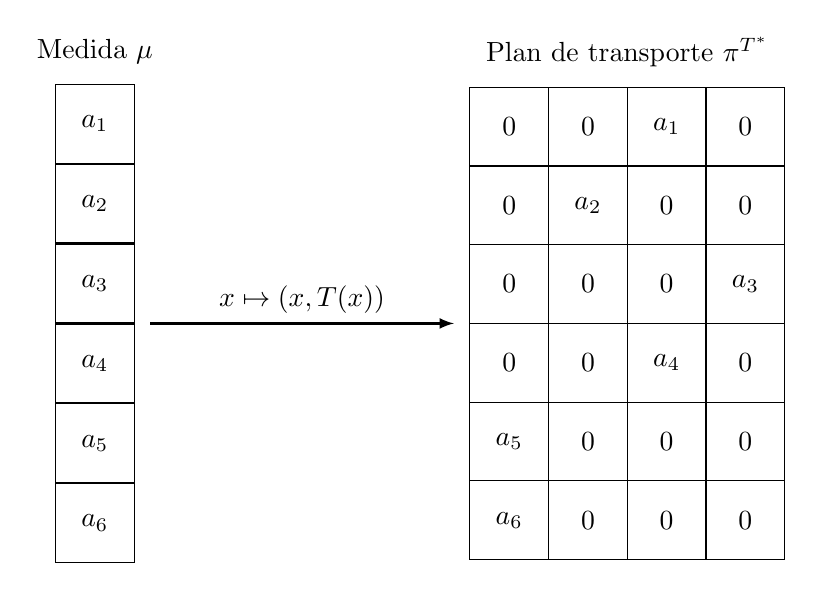
\begin{tikzpicture}[
        box/.style={draw, minimum size=1cm},
        arrow/.style={->, >=latex, shorten >=2pt, shorten <=2pt, thick}
    ]

    \matrix (D) [matrix of nodes, nodes={box}, column sep=-\pgflinewidth, label=above:Medida $\mu$] {
        $a_1$ \\
        $a_2$ \\
        $a_3$ \\
        $a_4$ \\
        $a_5$ \\
        $a_6$ \\
    };

    \matrix (C) [matrix of nodes, nodes={box, anchor=center}, column sep=-\pgflinewidth, row sep=-\pgflinewidth, right=4cm of D, label=above:Plan de transporte $\pi^{T^*}$] {
        0     & 0     & $a_1$ & 0     \\
        0     & $a_2$ & 0     & 0     \\
        0     & 0     & 0     & $a_3$ \\
        0     & 0     & $a_4$ & 0     \\
        $a_5$ & 0     & 0     & 0     \\
        $a_6$ & 0     & 0     & 0     \\
    };

    \draw[arrow] (D.east) -- node[midway, above] {$x \mapsto (x,T(x))$} (C.west);
\end{tikzpicture}

\end{document}